% Canonical editable Figure 1. Compile independently; main.tex embeds its PDF.
% Text follows spconf's Times family; mathematics retains Computer Modern,
% exactly as in the manuscript (newtxtext changes text only under XeTeX).
\documentclass[tikz,border=0pt]{standalone}
\usepackage{amsmath,amssymb,amsfonts,iftex}
\ifXeTeX
  \usepackage{newtxtext}
\else
  \renewcommand{\rmdefault}{ptm}
\fi
\usetikzlibrary{arrows.meta}
\definecolor{ink}{HTML}{18212B}
\definecolor{muted}{HTML}{485463}
\definecolor{frame}{HTML}{9AA6B2}
\definecolor{inputfill}{HTML}{F1F4F7}
\definecolor{inputedge}{HTML}{657381}
\definecolor{encoderfill}{HTML}{E8F2FB}
\definecolor{encoderedge}{HTML}{1477B8}
\definecolor{fusionfill}{HTML}{FFF3DF}
\definecolor{fusionedge}{HTML}{BC6A00}
\definecolor{outputfill}{HTML}{EEF7ED}
\definecolor{outputedge}{HTML}{39823D}
\definecolor{wireink}{HTML}{374553}
\tikzset{
  title/.style={anchor=base west,font=\fontsize{10.416bp}{12bp}\selectfont\bfseries,text=ink},
  role/.style={anchor=base west,font=\fontsize{9.072bp}{11bp}\selectfont\itshape,text=muted},
  label/.style={anchor=base,font=\fontsize{9.072bp}{11bp}\selectfont,text=ink},
  panel/.style={fill=white,draw=frame,line width=0.84bp,rounded corners=4.704bp},
  input/.style={fill=inputfill,draw=inputedge,line width=0.84bp,rounded corners=2.688bp},
  encoder/.style={fill=encoderfill,draw=encoderedge,line width=1.008bp,rounded corners=2.688bp},
  fusion/.style={fill=fusionfill,draw=fusionedge,line width=1.008bp,rounded corners=2.688bp},
  output/.style={fill=outputfill,draw=outputedge,line width=1.008bp,rounded corners=2.688bp},
  wire/.style={draw=wireink,line width=0.9408bp},
  arrow/.style={wire,-{Triangle[length=2.688bp,width=2.688bp]}}
}
\begin{document}
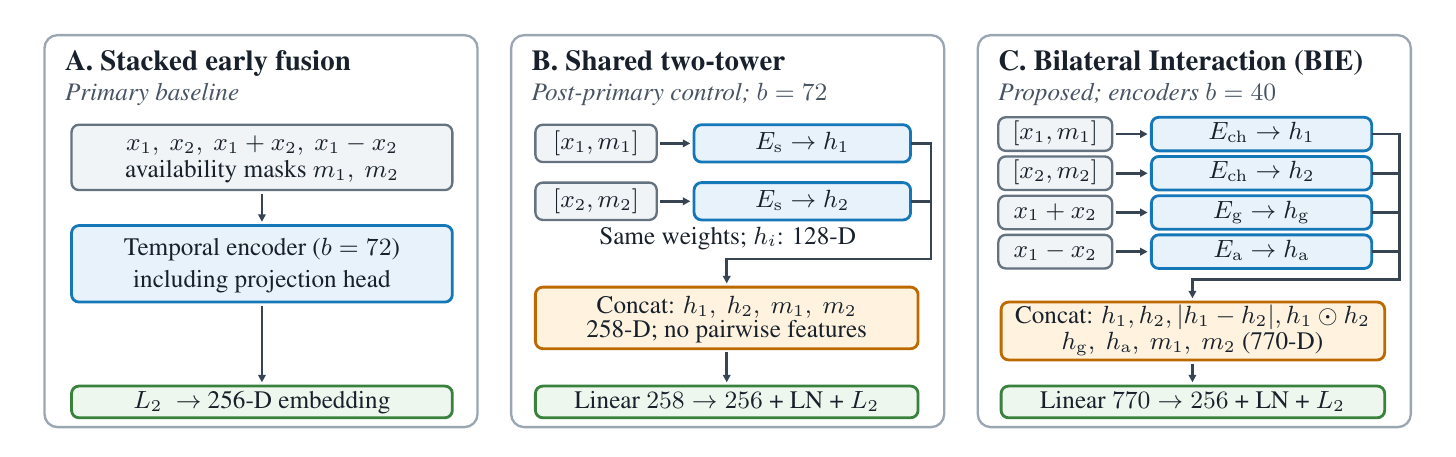
\begin{tikzpicture}[x=0.336bp,y=-0.336bp,every node/.style={inner sep=0pt,outer sep=0pt}]
\path[use as bounding box] (0,0) rectangle (1500,430);
\clip (0,0) rectangle (1500,430);

\draw[panel] (18,8) rectangle (482,428);
\node[title] (a-title) at (40,46) {A. Stacked early fusion};
\node[role] (a-role) at (40,78) {Primary baseline};
\draw[input] (47,104) rectangle (455,174);
\node[label] (a-input-1) at (251,132) {$x_1,\ x_2,\ x_1+x_2,\ x_1-x_2$};
\node[label] (a-input-2) at (251,161) {availability masks $m_1,\ m_2$};
\draw[arrow] (251,178) -- (251,208);
\draw[encoder] (47,212) rectangle (455,294);
\node[label] (a-encoder-1) at (251,244) {Temporal encoder ($b=72$)};
\node[label] (a-encoder-2) at (251,278) {including projection head};
\draw[arrow] (251,298) -- (251,380);
\draw[output] (47,384) rectangle (455,418);
\node[label] (a-output-1) at (251,408) {$L_2\ \rightarrow$ 256-D embedding};

\draw[panel] (518,8) rectangle (982,428);
\node[title] (b-title) at (540,46) {B. Shared two-tower};
\node[role] (b-role) at (540,78) {Post-primary control; $b=72$};
\draw[input] (544,104) rectangle (674,144);
\draw[input] (544,166) rectangle (674,206);
\node[label] (b-input-1) at (609,131) {$[x_1,m_1]$};
\node[label] (b-input-2) at (609,193) {$[x_2,m_2]$};
\draw[arrow] (678,124) -- (710,124);
\draw[arrow] (678,186) -- (710,186);
\draw[encoder] (714,104) rectangle (946,144);
\draw[encoder] (714,166) rectangle (946,206);
\node[label] (b-channel-1) at (830,131) {$E_{\mathrm{s}}\rightarrow h_1$};
\node[label] (b-channel-2) at (830,193) {$E_{\mathrm{s}}\rightarrow h_2$};
\node[label] (b-sharing) at (750,232) {Same weights; $h_i$: 128-D};
\draw[arrow] (946,124) -- (968,124) -- (968,248) -- (749,248) -- (749,274);
\draw[wire] (946,186) -- (968,186);
\draw[fusion] (544,278) rectangle (954,344);
\node[label] (b-concat-1) at (749,306) {Concat: $h_1,\ h_2,\ m_1,\ m_2$};
\node[label] (b-concat-2) at (749,332) {258-D; no pairwise features};
\draw[arrow] (749,348) -- (749,380);
\draw[output] (544,384) rectangle (954,418);
\node[label] (b-output-1) at (749,408) {Linear $258\rightarrow256$ + LN + $L_2$};

\draw[panel] (1018,8) rectangle (1482,428);
\node[title] (c-title) at (1040,46) {C. Bilateral Interaction (BIE)};
\node[role] (c-role) at (1040,78) {Proposed; encoders $b=40$};
\draw[input] (1040,96) rectangle (1162,132);
\draw[input] (1040,138) rectangle (1162,174);
\draw[input] (1040,180) rectangle (1162,216);
\draw[input] (1040,222) rectangle (1162,258);
\node[label] (c-input-1) at (1101,120) {$[x_1,m_1]$};
\node[label] (c-input-2) at (1101,162) {$[x_2,m_2]$};
\node[label] (c-input-g) at (1101,204) {$x_1+x_2$};
\node[label] (c-input-a) at (1101,246) {$x_1-x_2$};
\draw[arrow] (1166,114) -- (1200,114);
\draw[arrow] (1166,156) -- (1200,156);
\draw[arrow] (1166,198) -- (1200,198);
\draw[arrow] (1166,240) -- (1200,240);
\draw[encoder] (1204,96) rectangle (1440,132);
\draw[encoder] (1204,138) rectangle (1440,174);
\draw[encoder] (1204,180) rectangle (1440,216);
\draw[encoder] (1204,222) rectangle (1440,258);
\node[label] (c-channel-1) at (1322,120) {$E_{\mathrm{ch}}\rightarrow h_1$};
\node[label] (c-channel-2) at (1322,162) {$E_{\mathrm{ch}}\rightarrow h_2$};
\node[label] (c-global) at (1322,204) {$E_{\mathrm{g}}\rightarrow h_{\mathrm{g}}$};
\node[label] (c-asymmetry) at (1322,246) {$E_{\mathrm{a}}\rightarrow h_{\mathrm{a}}$};
\draw[arrow] (1440,114) -- (1470,114) -- (1470,270) -- (1248,270) -- (1248,290);
\draw[wire] (1440,156) -- (1470,156);
\draw[wire] (1440,198) -- (1470,198);
\draw[wire] (1440,240) -- (1470,240);
\draw[fusion] (1043,294) rectangle (1454,356);
\node[label] (c-concat-1) at (1248,317) {Concat: $h_1,h_2,\lvert h_1-h_2\rvert,h_1\odot h_2$};
\node[label] (c-concat-2) at (1248,345) {$h_{\mathrm{g}},\ h_{\mathrm{a}},\ m_1,\ m_2$ (770-D)};
\draw[arrow] (1248,360) -- (1248,380);
\draw[output] (1043,384) rectangle (1454,418);
\node[label] (c-output-1) at (1248,408) {Linear $770\rightarrow256$ + LN + $L_2$};
\end{tikzpicture}
\end{document}
